\documentclass[12pt, a4paper]{report}
\usepackage{graphicx}
\usepackage{ctex}
\usepackage[colorlinks=true]{hyperref}
\usepackage{indentfirst}
\usepackage{listings}
\graphicspath{{chapter/}{figures/}}
\usepackage{CJK}
\usepackage{tikz}
\usetikzlibrary{arrows,automata}
\usepackage{amsmath}

\usepackage{minted}

\begin{document} 
%%%%%%%%%%%%%%%%%%%%%%%%%%%%%%
%% 封面部分
%%%%%%%%%%%%%%%%%%%%%%%%%%%%%%
\begin{titlepage}
	\centering
	
\includegraphics[width=0.2\textwidth]{sf1.png}\par
	\vspace{1cm}
	
\includegraphics[width=0.8\textwidth]{sf.jpg}\par
	\vspace{0.1cm}
	{\scshape\LARGE Harbin Institute of Technology \par}
	\vspace{1cm}
	{\kaishu\LARGE 模式识别与深度学习\\实验报告\par}
	\vspace{1.5cm}
	{\huge\bfseries RNN网络函数预测与情感分析\par}
	\vspace{2cm}
	{\fangsong\Large\itshape 黄海\par}
	\vfill
	{1160300329}\par
	\fangsong{计算机科学与技术}
	\vfill
	指导教师	\textsc{左旺孟}
	\vfill
% Bottom of the page
	{\large \today\par}
\end{titlepage}



\sc
\tableofcontents
\newpage
\chapter{正弦预测}
\section{解释}

通过搭建基本的RNN网络,通过产生足够长度的时间序列,对每一组数据进行预测。这里采用的策略是把每个$2\pi$
分成两个部分,前一个部分进行训练,后一个部分进行预测,最后使用标准正弦进行拟合更正。

\section{代码}

以下是训练的部分代码
\small
\begin{minted}{python}

for step in range(200):
    start, end = step * np.pi, (step + 1) * np.pi
    steps = np.linspace(start, end, 5, dtype=np.float32)
    s.extend(steps)
    x_np = np.sin(steps - np.pi)
    y_np = np.sin(steps)
    x = Variable(torch.from_numpy(x_np[np.newaxis, :, np.newaxis]))
    y = Variable(torch.from_numpy(y_np[np.newaxis, :, np.newaxis]))
    prediction, self.h_state = self.module(x, self.h_state)
    p = prediction
    self.h_state = Variable(self.h_state.data)
    loss = self.loss_func(prediction, y)
    self.optimizer.zero_grad()
    loss.backward()
    self.optimizer.step()
    original_sin.extend(y_np.flatten())
    train_set.extend(prediction.data.numpy().flatten())

\end{minted}

\normalsize
\section{实验结果}

\begin{figure}[ht]
  \centering
  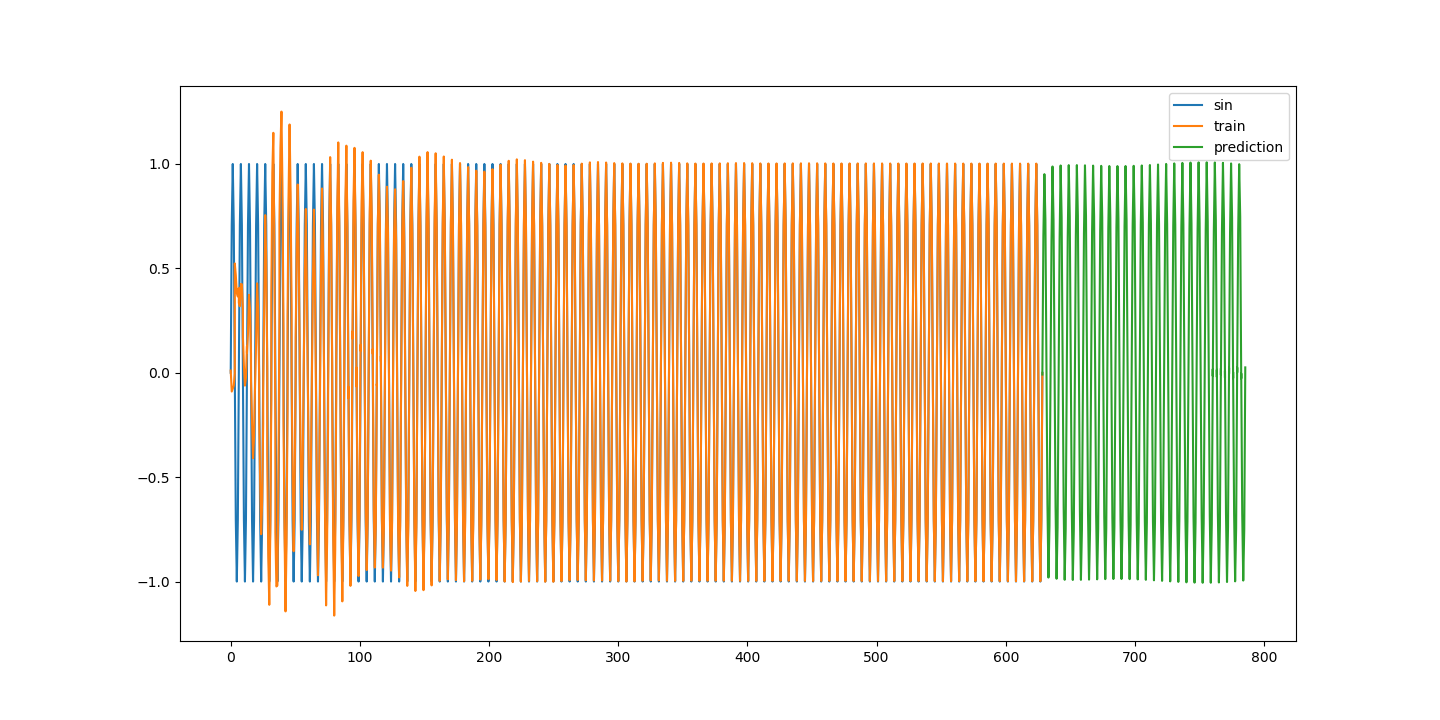
\includegraphics[scale=0.3]{Figure_1.png}
  \caption{训练以及预测结果}
  \label{}
\end{figure}

\chapter{文本情感分析}

\section{解释}

文本情感分析的主要难点在于如何组织数据并进行训练,在这次实验中,处理过后的数据分成了两块,前4000个语句为训练使用,后1000个为测试。
这之后便大同小异。调整好网络的参数,将输入调整为50个单词,对于不够长度的句子进行补齐。最后输出1维向量用来表示结果

\section{代码}

以下展示了部分的训练代码
\small
\begin{minted}{python}
for i in range(4000):
    print(i)
    x_np = np.array(self.negtrainnum[i])
    y_n = [self.negtrainlabels[i]]
    y_np = np.array(y_n)
    x_np = x_np.astype(np.float32)
    y_np = y_np.astype(np.float32)
    x = torch.from_numpy(x_np[np.newaxis, :])
    y = torch.from_numpy(y_np[np.newaxis, :, np.newaxis])
    x = Variable(x)
    y = Variable(y)
    prediction = self.module(x)
    loss = self.loss_func(prediction, y)
    self.optimizer.zero_grad()
    loss.backward()
    self.optimizer.step()
    # print(loss.item())

    x_np = np.array(self.postrainnum[i])
    y_n = [self.postrainlabels[i]]
    y_np = np.array(y_n)
    x_np = x_np.astype(np.float32)
    y_np = y_np.astype(np.float32)
    x = torch.from_numpy(x_np[np.newaxis, :])
    y = torch.from_numpy(y_np[np.newaxis, :, np.newaxis])
    x = Variable(x)
    y = Variable(y)
    prediction = self.module(x)
    loss = self.loss_func(prediction, y)
    self.optimizer.zero_grad()
    loss.backward()
    self.optimizer.step()
    # print(loss.item())
print("End Train.")
\end{minted}
\normalsize

\end{document}
